\documentclass[12pt]{article}

\usepackage{amsmath, amssymb, amsfonts, setspace, stmaryrd, amsthm, graphicx, tikz}
\usepackage[utf8]{inputenc}
\usepackage[english]{babel}
\usetikzlibrary{positioning}% To get more advances positioning options
\usetikzlibrary{arrows}% To get more arrow heads

\usepackage[margin=1in]{geometry}
\newtheorem{theorem}{Theorem}

%%align* environment
\newcommand{\eq}[1]{\begin{align*}#1\end{align*}}

%Math commands
\DeclareMathOperator{\R}{\mathbb{R}}
\DeclareMathOperator{\C}{\mathbb{C}}
\DeclareMathOperator{\Z}{\mathbb{Z}}
\DeclareMathOperator{\N}{\mathbb{N}}
\DeclareMathOperator{\Q}{\mathbb{Q}}

\newcounter{exercise}[section]
\newenvironment{exercise}[1][]{\refstepcounter{exercise}\par\medskip
	\noindent \textbf{Exercise~\thesection.\theexercise #1} \rmfamily}{\medskip}

\title{Girls Talk Math: \\Networks Group}
\author{}
\date{}

\begin{document}

\maketitle

\section{Introduction}
By this point in high school, you've probably taken a lot of classes on math--pre-algebra, algebra, geometry, algebra II, calculus, etc. etc. And it might seem like everything at this point is about how we manipulate equations and understand functions. What we're going to teach you here probably will seem different--and maybe not like any of the math you've seen before, but requires the same amount of rigor and has the same usefulness. 
\\
To start out with, we define a \emph{graph} not as a relation between a domain and range in Euclidean space, but as a structure in which certain pairs of objects are related to one another and others aren't. These objects are called \emph{vertices} (or nodes) and the relations are called \emph{edges} (or links). If these vertices represent some kind of meaningful data (and perhaps contain \emph{attributes}), then we typically call the graph a \emph{network} (the terms are often used interchangeably. Such networks are used in social media and business (predicting suggestions for 'who to follow on instagram, or what books you might like to buy on Amazon), as well as in physical/biological sciences (mapping what regions function together in the brain).
\section{Graph Theory}
\emph{Graph theory} is the mathematical study of (wait for it) graphs. Let's begin our study by labeling the edges and vertices of a particular simple graph (below).

\begin{figure}[htbp]
\begin{center}
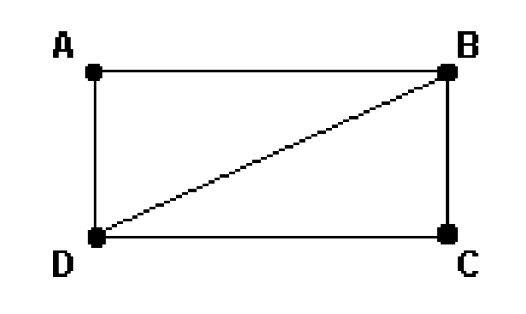
\includegraphics[]{abcd.png}
\caption{A simple graph}
\label{default}
\end{center}
\end{figure}

We use letters in this depiction, but these could in general be numbers, names, etc. The vertices here are \emph{A}, \emph{B}, \emph{C}, and \emph{D}. The edges are \emph{AB}, \emph{BC}, \emph{CD}, \emph{AD}, and \emph{BD}. If two nodes share an edge, they are said to be \emph{adjacent}. When we list these vertices, the order is not important---\emph{BD} is the same edge as \emph{DB}---in general, this is not always true, but it is true for \emph{undirected} graphs, which are the ones we will study here. Notice also that nodes \emph{A} and \emph{C} are adjacent to two edges each--but \emph{B} and \emph{D} are each adjacent to two three edges. The number of edges adjacent to a particular node is called that node's \emph{degree} (so \emph{A} has degree 2, etc.)

In the previous graph (Fig. 1), one would travel from node \emph{A} to each other node in the graph, through its edges. If this is true, the graph is said to be \emph{connected}. In the graph below (Fig. 2), the graph is disconnected, as \emph{F} and \emph{G} cannot be reached (through traveling via edges) from the rest of the graph.

\begin{figure}[htbp]
\begin{center}
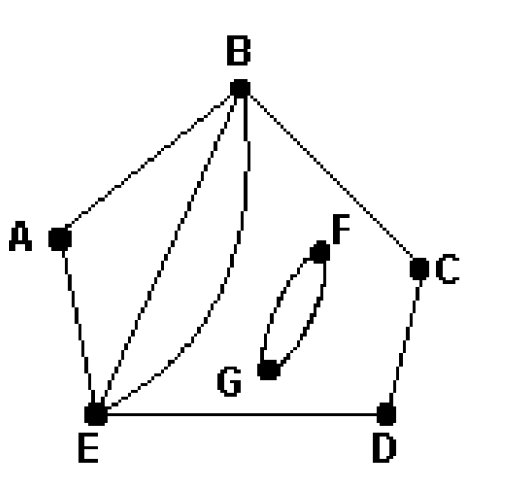
\includegraphics[]{disconnected.png}
\caption{A disconnected graph}
\label{default}
\end{center}
\end{figure}

If a graph is disconnected, we can divide it into \emph{components}. Each connected subgraph is called a component--in the above graph, \emph{F}, \emph{G}, and the corresponding edges form one component; \emph{A}, \emph{B}, \emph{C}, \emph{D}, \emph{E}, \emph{F}, and the corresponding edges form the other component. Saying that a graph is connected is equivalent to saying that it has one component. \emph{Important: Saying that two nodes are adjacent is more specific than saying they are connected (these are frequently confused).}

\begin{exercise}
For each figure below, list the vertices and their degrees, as well as the edges. Decide whether of not the graph is connected--if it is not, how many components does it have.

{\bf 1.}
\begin{tikzpicture}[>=triangle 45,font=\sffamily]
    \node (X) at (0,0) {x};
    \node (Y) [below left=2cm and 1cm of X]  {y};% 2cm below, 1cm to the left (optional)
    \node (Z) [below right=2cm and 1cm of X] {z};
    \node (U) [below left=2cm and 1cm of Z]  {u};
    \draw [semithick,-] (X) -- (Y);
    \draw [semithick,-] (X) -- (Z);
    \draw [semithick,-] (Y) -- (U);
    \draw [semithick,-] (Z) -- (U) ;
\end{tikzpicture}
{\bf 2.}
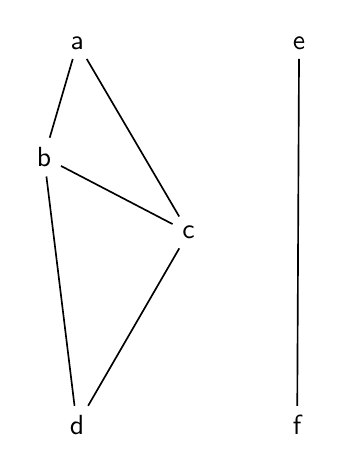
\begin{tikzpicture}[>=triangle 45,font=\sffamily]
    \node (A) at (0,0) {a};
    \node (B) [below left=1cm and 0cm of A]  {b};% 2cm below, 1cm to the left (optional)
    \node (C) [below right=2cm and 1cm of A] {c};
    \node (D) [below left=2cm and 1cm of C]  {d};
    \node (F) [below right=2cm and 1cm of C]  {f};
	\node (E) [above right=2cm and 1cm of C]  {e};

    \draw [semithick,-] (A) -- (B);
    \draw [semithick,-] (B) -- (C);
    \draw [semithick,-] (A) -- (C);
    \draw [semithick,-] (B) -- (D);
    \draw [semithick,-] (C) -- (D) ;
    \draw [semithick,-] (E) -- (F) ;
\end{tikzpicture}
{\bf 3.}
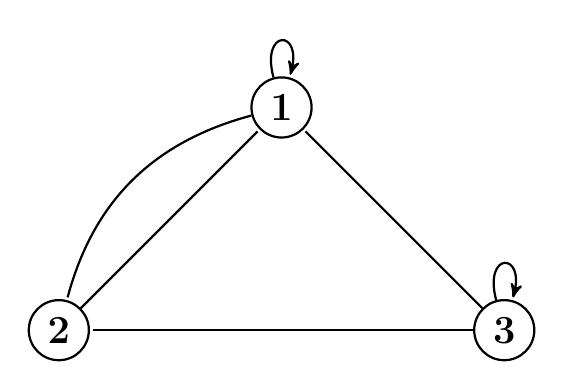
\begin{tikzpicture}[-,>=stealth',shorten >=1pt,auto,node distance=4cm,
                thick,main node/.style={circle,draw,font=\Large\bfseries}]

  \node[main node] (1) {1};
  \node[main node] (2) [below left of=1] {2};
  \node[main node] (3) [below right of=1] {3};

  \path
    (1) edge [loop above] (1)
        edge [bend right] (2)
    (2) edge [below] (1)
    (3) edge [loop above] (3)
        edge [right]  (1)
        edge [below]  (2);      
\end{tikzpicture}
\\
\\
{\bf 1. Nodes and their degrees:}
\\
\\
{\bf Edges:}
\\
\\
{\bf Connected?}
\\
{\bf Components:}
\\
\\
{\bf 2. Nodes and their degrees:}
\\
\\
{\bf Edges:}
\\
\\
{\bf Connected?}
\\
{\bf Components:}
\\
\\
{\bf 3. Nodes and their degrees:}
\\
\\
{\bf Edges:}
\\
\\
{\bf Connected?}
\\
{\bf Components:}
\\
\\
\end{exercise}

Were you confused on  the last exercise? This was admittedly intentional. Nodes 1 and 3 each have an edge unto themselves--also called a \emph{loop} (or self-edge). These contribute two to their degree (so node 1 has degree  5 and node 3 has degree 4). Also, this graph has two edges from node 1 to node 2 (\emph{12})---a graph with multiple edges between the same pair of nodes is called a \emph{multigraph}.
\subsection{Euler Paths and Euler Circuits}
An important question in mathematics was asked to Leonhard Euler in the late 1700s in the city of Königsberg, Prussia. Using the map of the city below, he was asked, is there some route in the city wherein one would cross each of the seven bridges once and only once?
\begin{figure}[htbp]
\begin{center}
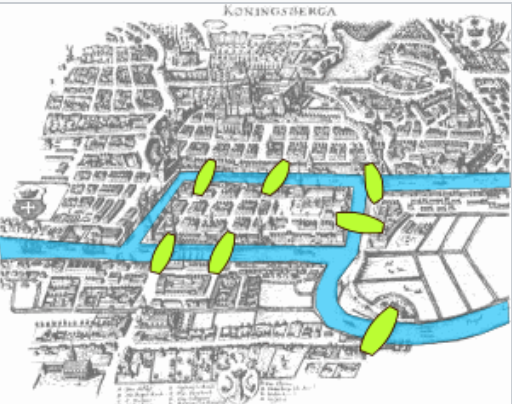
\includegraphics[]{euler.png}
\caption{A map of the city of Königsberg, showing the seven bridges and the land masses which they connect.}
\label{default}
\end{center}
\end{figure}
Now, this may not seeem to have to anything to do with graph theory, but it in fact led to the first journal article in the subject. He redrew the figure above as a graph, considering the land masses to be vertices and the bridges to be edges.
\begin{exercise}
Using the above reasoning, recreate Euler's representation of Königsberg. Label the degree of each node.
\\
\\
\\
\\
\\
\\
\\
\end{exercise}
Now, with this tool, the problem is not so hard---the problem can be restated: are there any paths through the graph such that one crosses all of the edges once and only once. Upon careful consideration, you may see that even degree vertices are useful to this determination---in a degree 2 vertex, one can enter and leave the vertex through two edges (if it is four, this can happen twice, etc.) But with odd degree nodes, one may get 'stuck' at the vertex. In fact, for there to be such a path through the graph as Euler desired, there must be two or less odd  degree vertices. Such a path is named an \emph{Euler path}.  Because, as you showed above, there are more than two vertices of odd degree in the Königsberg graph, there are no Euler paths in the associated city.
\begin{theorem}
In order for there to be an Euler path (in which each edge is traversed exactly once) in a graph, that graph must be connected and have two or less vertices of odd degree. If we restrict the path to circuits (in which the path must end at the same point at which it starts), the graph must have exactly zero vertices of odd degree (and must be connected). Such a path is called an Euler circuit or Eulerian cycle.
\end{theorem}
\begin{exercise}
Do the graphs from Excercise 2.1 have Euler paths? Euler circuits? Why or why not?
{\bf 1.}
\begin{tikzpicture}[>=triangle 45,font=\sffamily]
    \node (X) at (0,0) {x};
    \node (Y) [below left=2cm and 1cm of X]  {y};% 2cm below, 1cm to the left (optional)
    \node (Z) [below right=2cm and 1cm of X] {z};
    \node (U) [below left=2cm and 1cm of Z]  {u};
    \draw [semithick,-] (X) -- (Y);
    \draw [semithick,-] (X) -- (Z);
    \draw [semithick,-] (Y) -- (U);
    \draw [semithick,-] (Z) -- (U) ;
\end{tikzpicture}
{\bf 2.}
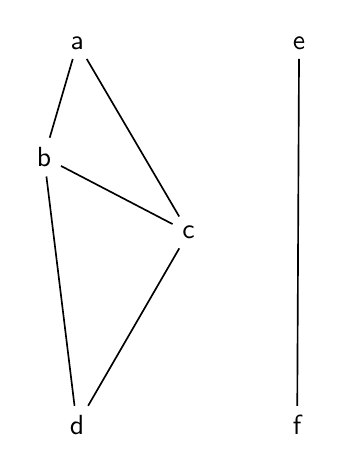
\begin{tikzpicture}[>=triangle 45,font=\sffamily]
    \node (A) at (0,0) {a};
    \node (B) [below left=1cm and 0cm of A]  {b};% 2cm below, 1cm to the left (optional)
    \node (C) [below right=2cm and 1cm of A] {c};
    \node (D) [below left=2cm and 1cm of C]  {d};
    \node (F) [below right=2cm and 1cm of C]  {f};
	\node (E) [above right=2cm and 1cm of C]  {e};

    \draw [semithick,-] (A) -- (B);
    \draw [semithick,-] (B) -- (C);
    \draw [semithick,-] (A) -- (C);
    \draw [semithick,-] (B) -- (D);
    \draw [semithick,-] (C) -- (D) ;
    \draw [semithick,-] (E) -- (F) ;
\end{tikzpicture}
{\bf 3.}
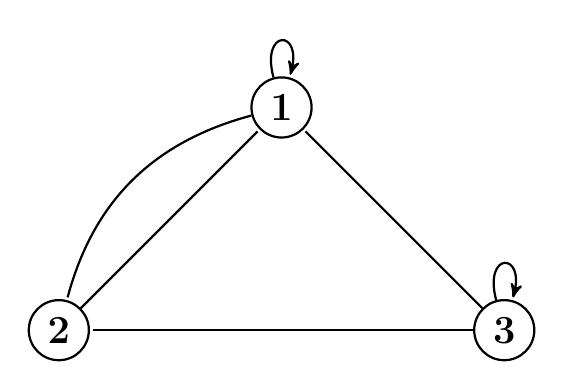
\begin{tikzpicture}[-,>=stealth',shorten >=1pt,auto,node distance=4cm,
                thick,main node/.style={circle,draw,font=\Large\bfseries}]

  \node[main node] (1) {1};
  \node[main node] (2) [below left of=1] {2};
  \node[main node] (3) [below right of=1] {3};

  \path
    (1) edge [loop above] (1)
        edge [bend right] (2)
    (2) edge [below] (1)
    (3) edge [loop above] (3)
        edge [right]  (1)
        edge [below]  (2);      
\end{tikzpicture}
\\
\\
1. Euler circuit, Eulter path, or neither?\\
Why?\\
\\
\\
Can you draw the circuit/path if there is one? (Do so on the graph)
\\
\\
\\
2. Euler circuit, Eulter path, or neither?\\
Why?\\
\\
\\
Can you draw the circuit/path if there is one? (Do so on the graph)
\\
\\
\\
3. Euler circuit, Eulter path, or neither?\\
Why?\\
\\
\\
Can you draw the circuit/path if there is one? (Do so on the graph)
\\
\\
\\
\end{exercise}
In the questions above, we asked you to draw the Euler circuits/paths without any prescribed method. For larger graphs, this is actually quite hard to do from guessing---however, there is a method known a \emph{Fleury's algorithm} for doing this (we skip this in favor of learning some more interesting things later, but when we input graphs into Mathematica, this is the method that the software uses).
\subsection{Other Results from Graph Theory}
Before we move onto programming with graphs, we discuss a few other results from graph theory. The first term we will define is a \emph{complete graph}, which is a graph in which each node is adjacent to every other node in the graph. Can you guess how many edges are in this graph?
\\
To start you off, there are $n$ nodes in the graph. How many edges do each of these nodes share? \underline{\hspace{2cm}}. After we account for the fact that this counts each node twice, we see that there are \underline{\hspace{3cm}} edges in the complete graph.
\\
The complete graph on $n$ nodes is often denoted by $K_n$. As we show below, $K_2$ is just an edge shared by two vertices, $K_3$ is a triangle, and $K_4$ is a rectangle with diagonals. These graphs have $2(2-1)/2=1$, $3(3-1)/2=3$, and $4(4-1)/2=6$ edges, as we show below.
\\
\begin{figure}[htbp]
\begin{center}
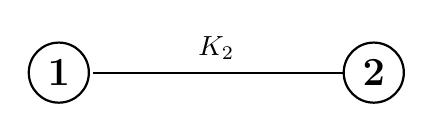
\begin{tikzpicture}[-,>=stealth',shorten >=1pt,auto,node distance=4cm,
                thick,main node/.style={circle,draw,font=\Large\bfseries}]

  \node[main node] (1) {1};
  \node[main node] (2) [right of=1] {2};
  \node[align=center,font=\bfseries, yshift=2em] (title) 
    at (current bounding box.south)
    {$K_2$};

  \path
    (2) edge [right] (1);
    
\end{tikzpicture}  
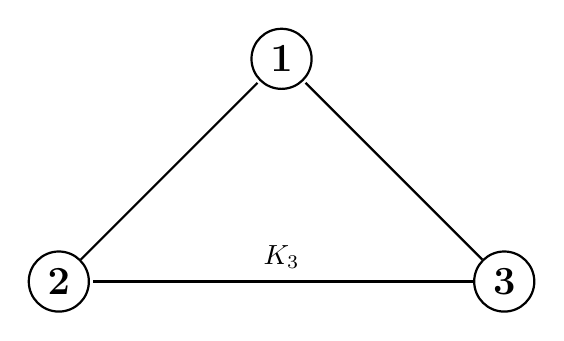
\begin{tikzpicture}[-,>=stealth',shorten >=1pt,auto,node distance=4cm,
                thick,main node/.style={circle,draw,font=\Large\bfseries}]

  \node[main node] (1) {1};
  \node[main node] (2) [below left of=1] {2};
  \node[main node] (3) [below right of=1] {3};
  \node[align=center,font=\bfseries, yshift=2em] (title) 
    at (current bounding box.south)
    {$K_3$};

  \path
    (2) edge [below] (1)
    (3) edge [right]  (1)
        edge [below]  (2);      
\end{tikzpicture}
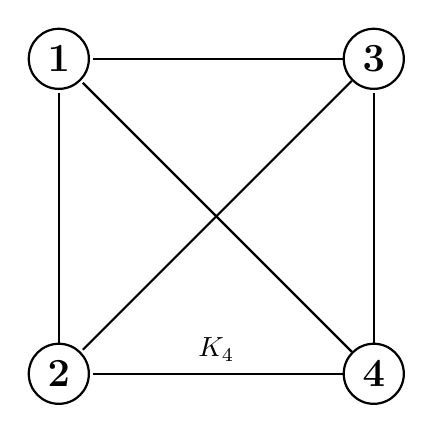
\begin{tikzpicture}[-,>=stealth',shorten >=1pt,auto,node distance=4cm,
                thick,main node/.style={circle,draw,font=\Large\bfseries}]

  \node[main node] (1) {1};
  \node[main node] (2) [below of=1] {2};
  \node[main node] (3) [right  of=1] {3};
  \node[main node] (4) [right  of=2] {4};
  \node[align=center,font=\bfseries, yshift=2em] (title) 
    at (current bounding box.south)
    {$K_4$};

  \path
  	(4) edge [below]  (3)
    (2) edge [below]  (1)
    (3) edge [right]  (1)
        edge [below]  (2)
    (4) edge [right]  (2)
        edge [right]  (1);
    
\end{tikzpicture}
\end{center}
\end{figure}
In addition to compelte graphs, we have \emph{regular graphs}, graphs in which each vertex has the same degree. Regular graphs may or may not be complete, but complete graphs are always regular---for example, each node in $K_3$ has degree $2$ and each node in $K_4$ has degree $3$. Below, we show the 2-regular graph on 4 nodes, which is simply a rectangle.
\begin{figure}[htbp]
\begin{center}
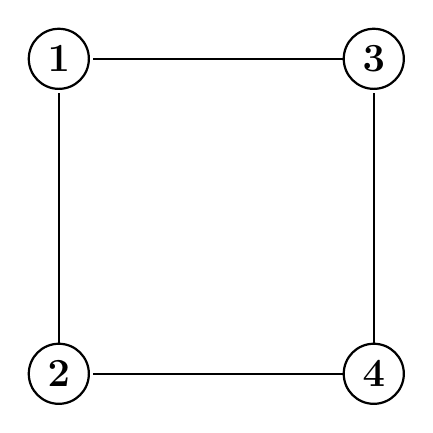
\begin{tikzpicture}[-,>=stealth',shorten >=1pt,auto,node distance=4cm,
                thick,main node/.style={circle,draw,font=\Large\bfseries}]

  \node[main node] (1) {1};
  \node[main node] (2) [below of=1] {2};
  \node[main node] (3) [right  of=1] {3};
  \node[main node] (4) [right  of=2] {4};
  

  \path
    (2) edge [below]  (1)
    (3) edge [right]  (1)
    (4) edge [below]  (3)
    (4) edge [right]  (2);
    
\end{tikzpicture}
\end{center}
\end{figure}
\begin{exercise}
\\1. Draw a 1-regular graph on four vertices. Is it connected?
\\
\\
\\
\\
\\
\\
\\
\\
2. Is there a 1-regular graph on three vertices? If not, can you explain why?
\\
\\
\\
\\
\\
\\
3. Draw $K_5$. How many edges does it have?
\\
\\
\\
\\
\\
\\
\\
\\
4. Does $K_3$ have an Euler circuit or path? What about $K_4$? $K_5$? Can you make a statement about which complete graphs have Euler circuits/paths and which do not?
\\
\\
\\
\\
\\
\\
\\
\end{exercise}
\subsection{Computing with graphs in Mathematica}
At this point, most of the tools we will learn are more relevant to larger graphs and data analysis, which makes paper computation difficult. Therefore, we're going to learn some basic graph computation in Mathematica. In this section, we cover how to input a graph, how to draw a graph, how to compute the degrees of a graph's vertices, and how to compute it's Euler circuits/paths.
\\
An \emph{edgelist} is the primary tool for graph data in mathematica. It is simply the list of edges in the graph. For example, an edgelist for $K_3$ would be $1-2$, $1-3$, $2-3$.
To input this in Mathematica, we type "Graph[{1<->2,2<->3,1<->3}]". We may also explicitly list the vertices--say we want to input the previous graph, but also list a fourth vertex not connected to the other three. Then we could input "Graph[{1,2,3,4},{1<->2,2<->3,1<->3}]". In general, the format is "Graph[{$v_1,v_2,..v_n$},{$e_1,...,e_m$}]". We may also modify the edge and vertex colors, as well as list the vertex names i.e. "Graph[{1,2,3,4},{1<->2,2<->3,1<->3},VertexStyle->Green,EdgeStyle->Blue,VertexLabel->"Name"]". We could also use letters or names instead of numbers i.e. "Graph[{A<->Francesca, B<->Katrina,B<->A}]".
\\
We can save the triangle graph by inputting "g="Graph[{1,2,3,4},{1<->2,2<->3,1<->3}]". This allows us to get the degrees of each vertex by inputting "VertexDegree[g]".\\
Mathematica 'knows' certain types of graphs--i.e. the octahedral graph, a 4-regular graph on 6 vertices. To find its Eulerian cycles, first type "g=GraphData["OctahedralGraph"];" and then "FindEulerianCycle[g]".
\begin{exercise}\\
1. The Harary graph $H_{k,n}$ is a connected graph in which each of $n$ nodes has at least degree $k$---this is very similar to a $k$ regular graph. In many cases, they are equivalent, but in cases where the $k$ regular graph on $n$ vertices does not exist (i.e. number 2 of the previous exercise set)--in these cases, the Harary graph is the closest thing. First, construct the Harary graph $H_{3,5}$ by inputting "g=HararyGraph[3,5]". Find the degrees of its vertices and draw below, listing these degrees.
\\
\\
\\
\\
\\
\\
2. Construct the complete graph on $7$ vertices by inputting "g=Completegraph[7,VertexLabel$->$"Name"]". Find one of its Eulerian cyclces. To show the steps of the cycle, type "Table[HighlightGraph[G,Part[First[\%],1;;i]],{i,Length[First[\%]]}]". What is the first edge traversed?
\\
\\
The last?
\\
\end{exercise}
\\At this point, students should complete the "Graph Theory Additional Questions" worksheet.
\section{Network Theory}
In the previous section, we presented a quick survey of classical graph theory. We hope this was interesting in its own right, but here we change our direction and shift more to the application-based study of graphs, which is often called \emph{network theory}. Most of the exercises for this section will be in mathematica, as the computations involved are relatively hard and sometimes require \emph{probabilistic calculations}.
\subsection{Random Graphs}
Thus far, we have considered regular and complete graphs---while these are new to you, they are relatively boring to the well-studied mathematician. Most network studies involve some variatio of \emph{random graphs}, which are graphs generated from probabilistic calculations. For example, a particular random graph might be generated by placement of $10$ edges at random between $8$ nodes, so that nodes $A$ and $B$ share an edge with the same probability as any other two nodes in the graph. This type of graph, in which $m$ edges are randomly placed between $n$ nodes, is called an Erdős-Renyí (E-R) graph, and is denoted by $G(n,m)$.
\\
However, E-R graphs are really just the start of random graphs. Two other types of commonly used networks are referred to as the \emph{Barabási-Albert (BA) model} and the \emph{Watts Strogatz (WS) model}. \\Graphs of the BA type are generated from a 2-regular graph, adding $n$ nodes and $k$ vertcies at each step, but in such a way that the probability of an edge being added to a particular vertex is proportional to that vertex's degree at the step. This process creates a wide \emph{degree distribution}, such that some nodes have very high degrees while others have very low degrees---in particular, BA graphs have been shown to be good models for many applications. The most famous example of this is in internet linkages across the web---highly visited and linked to webpages will tend to get more and more traffic over time, so that yet more sites will link to them i.e. \emph{the rich get richer}. If a site is less linked to, then fewer visitors will see the site and link to it in the future. This creates the wide degree distribution seen in BA networks. Another example relevant to the BA model is the use of different food items in recipe databases (See Figure).
\begin{figure}[htbp]
\begin{center}
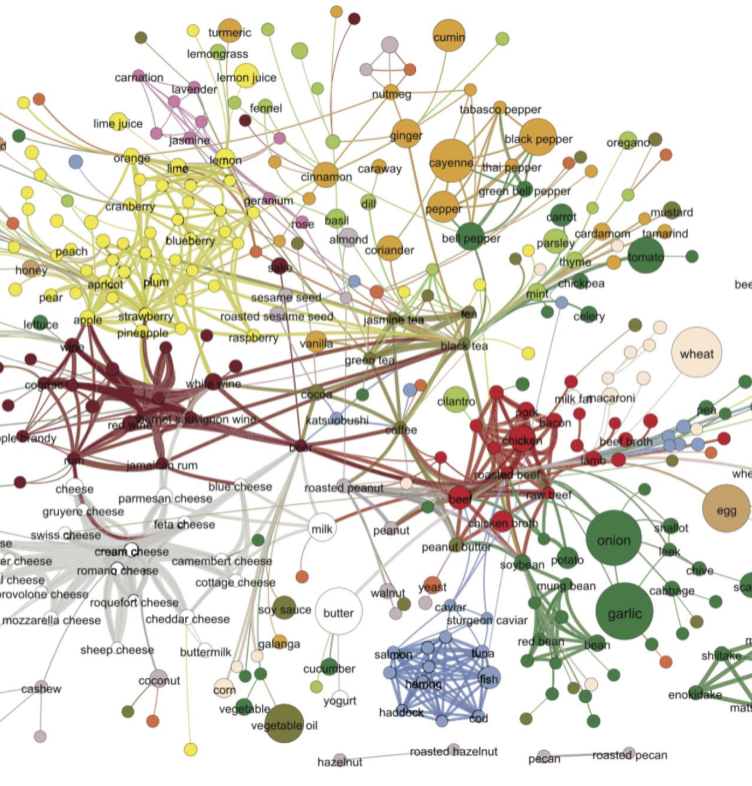
\includegraphics[]{foodnet.png}
\caption{The size of each node represents how many recipes it is given in, while the thickness of an edge between two nodes represents the number of recipes featuring the two adjacent nodes together (Figure from blog: ScienceandFood).}
\label{default}
\end{center}
\end{figure}
 

\begin{exercise}
1. Create an Erdős-Renyí graph of $20$ edges on $18$ nodes $G(18,20)$ in Mathematica by inputting "g1=RandomGraph[{18,20}]". Draw your graph here, and compare with someone around you.
\\
\\
\\
\\
\\
\\
2. Compute the average of the degrees of the vertices in your graph $G(18,20)$ (usually we call this the \emph{mean degree}). Is this the same as what people around you got?
\\
\\
\\
\\
\\
3. Can you come up with a formula for the mean degree of $G(m,n)$ given $m$ and $n$.
\\
\\
\\
\\
4. Construct a BA graph on $10$ vertices by inputting  "g2=RandomGraph[BarabasiAlbertGraphDistribution[10,2]]". How does this compare in your own words to the random graph from question 1.
\\
\\
\\
\\
\\
\end{exercise}
We can give better illustration of the \emph{degree distributions} by showing them in plot form. This is a bit advanced for those who have not had a statistics course, but hopefully we can teach you what these plots mean. Look at Figure .  The horizontal axes represent the degree $d$. See that this varies between and. The vertical axis represent the \emph{Probability of having degree d}. You can see that one either plot, there is a high probability that a node has degree $d=$, but this is much higher on the right plot.
\subsection{Other Network Properties: Centrality and Clustering Coefficient}
We have already seen several important properties in action---the number of components tells us 'how many pieces' a network comes in. The mean degree tell us how densely connected a network is. And the degree distribution gives us an idea of the variation within the network. A different kind of property, called \emph{centrality}, tells us about the relative importance of each node within its network.\\
The first kind of centrality is very simple and intuitive. A node's \emph{Degree Centrality} is simply the degree of that node $d$, divided by  its maximum possible degree, which is $m-1$, where $m$ is the number of edges in the network. A high degree node is usually an important player in the network--for example, garlic's use in the food network above has a high degree because it is used frequently in lots of networks. In friendship networks, the most popular units have the highest degrees, etc.\\
Now, to get an idea of the second type of centrality, think of Washington DC's subway system (or any other city's subway system). There are certain stops that several lines go through, and consequentially many passengers on different lines go through these stops (see Figure \ref{subway}). A node's \emph{Betweenness centrality} captures this, by taking into account how many shortest paths between different nodes in the network pass through the node of interest. 
\begin{figure}[htbp]
\begin{center}
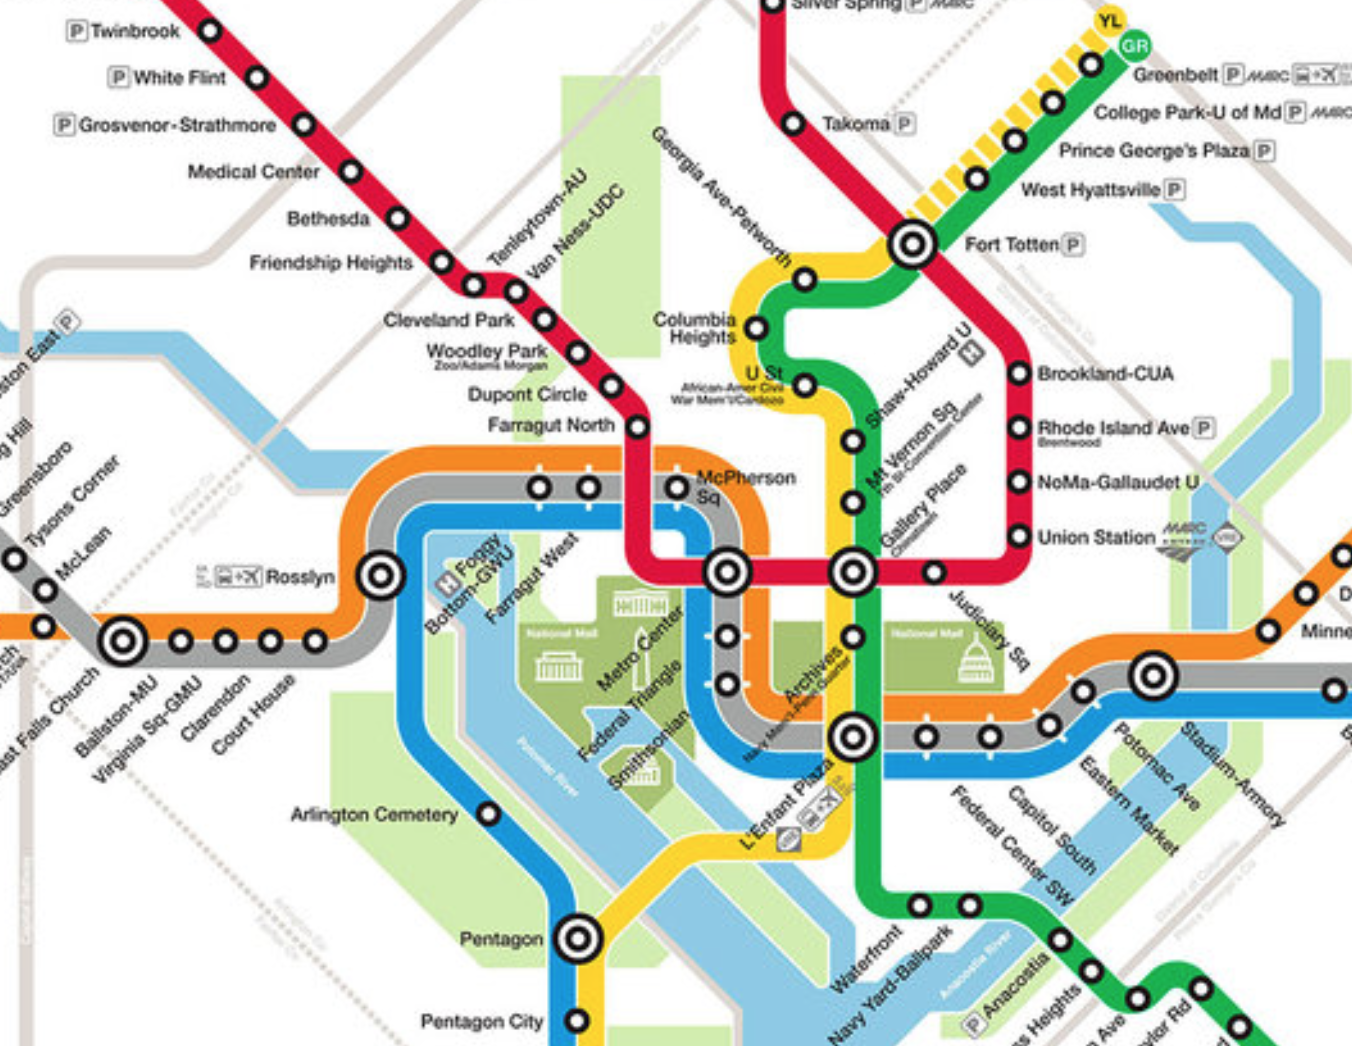
\includegraphics[width=.8\linewidth]{subway.png}
\caption{If we consider the network wherein each stop in a node, and the paths between them are edges, nodes like Gallery Place (or L'Enfants Plaza) are important because they lie on the shortest path of many routes (ie from Judiciary Square to Metro Center, or to Archives). Gallery Place also has a relatively high degree, but betweenness centrality better captures its importance in the network, and would be more useful to engineers considering subway station repairs/closures.}
\label{subway}
\end{center}
\end{figure}

Unfortunately, this calculation is much longer and more complicated. For a connected network, it is defined as the number of shortest paths passing through the node, divided by the total number of shortest paths in the network, \emph{taking into account every pair of nodes in the network.} We will calculate this for one small network, and then let mathematica take it from there. \\
Examine Figure \ref{bw}, and consider node $1$--what shortest paths pass through it? Well, a shortest path from 2 to 5 passes through it (2-1-5), and this is the only shortest path from 2 to 5--this contributes $1/1=1$ to the calculation.. The same can be said for 3 to 5. As well, both paths from 4 to 5 pass through 1 (the 'top' way 5-1-3-4 and the bottom way 5-1-2-4), and this also contributes $2/2=1$. How about shortest paths form $2$ to $3$? One (2-1-3) of these goes through $1$ while the other goes through $4$ (2-1-4), so this contributes $1/2$ to the calculation.. Do any paths from 3 to 2 pass through it? No--therefore, we've considered all pairs of nodes and the shortest paths passing through $1.$ Adding up the contributions we found, we get $1+1+1+1/2=3.5$. Now we divide this by the number of pairs in the graph which exclude $1$---there are six of these (5-3,5-2,5-4,2-3,2-4,3-4), and find that the betweenness centrality of $1$ is $3.5/6=0.58$.
\begin{figure}[htbp]
\begin{center}
\begin{tikzpicture}[-,>=stealth',shorten >=1pt,auto,node distance=4cm,
                thick,main node/.style={circle,draw,font=\Large\bfseries}]

  \node[main node] (1) {1};
  \node[main node] (2) [below right of=1] {2};
  \node[main node] (3) [above right of=1] {3};
  \node[main node] (4) [above right of=2] {4};
  \node[main node] (5) [left of=1] {5};
  

  \path
    (2) edge [below]  (1)
    (3) edge [right]  (1)
    (4) edge [below]  (3)
    (4) edge [right]  (2)
    (5) edge [left] (1);
    
\end{tikzpicture}
\label{bw}
\caption{Betweenness Centrality example}
\end{center}
\end{figure}
There are \emph{many} other types of centrality, but only so little time (and many of these methods require exposure to math that most of you have probably not yet learned)---indeed, Google uses a variant of something called 'eigenvector centrality' to rank the results of our web searches. However, these two kinds of centrality we've covered are among the most important and will suffice for our study.
\begin{exercise}
1. Consider the graph below. Which node(s) have the highest degree centrality? Which do think has/have the highest betweenness centrality?

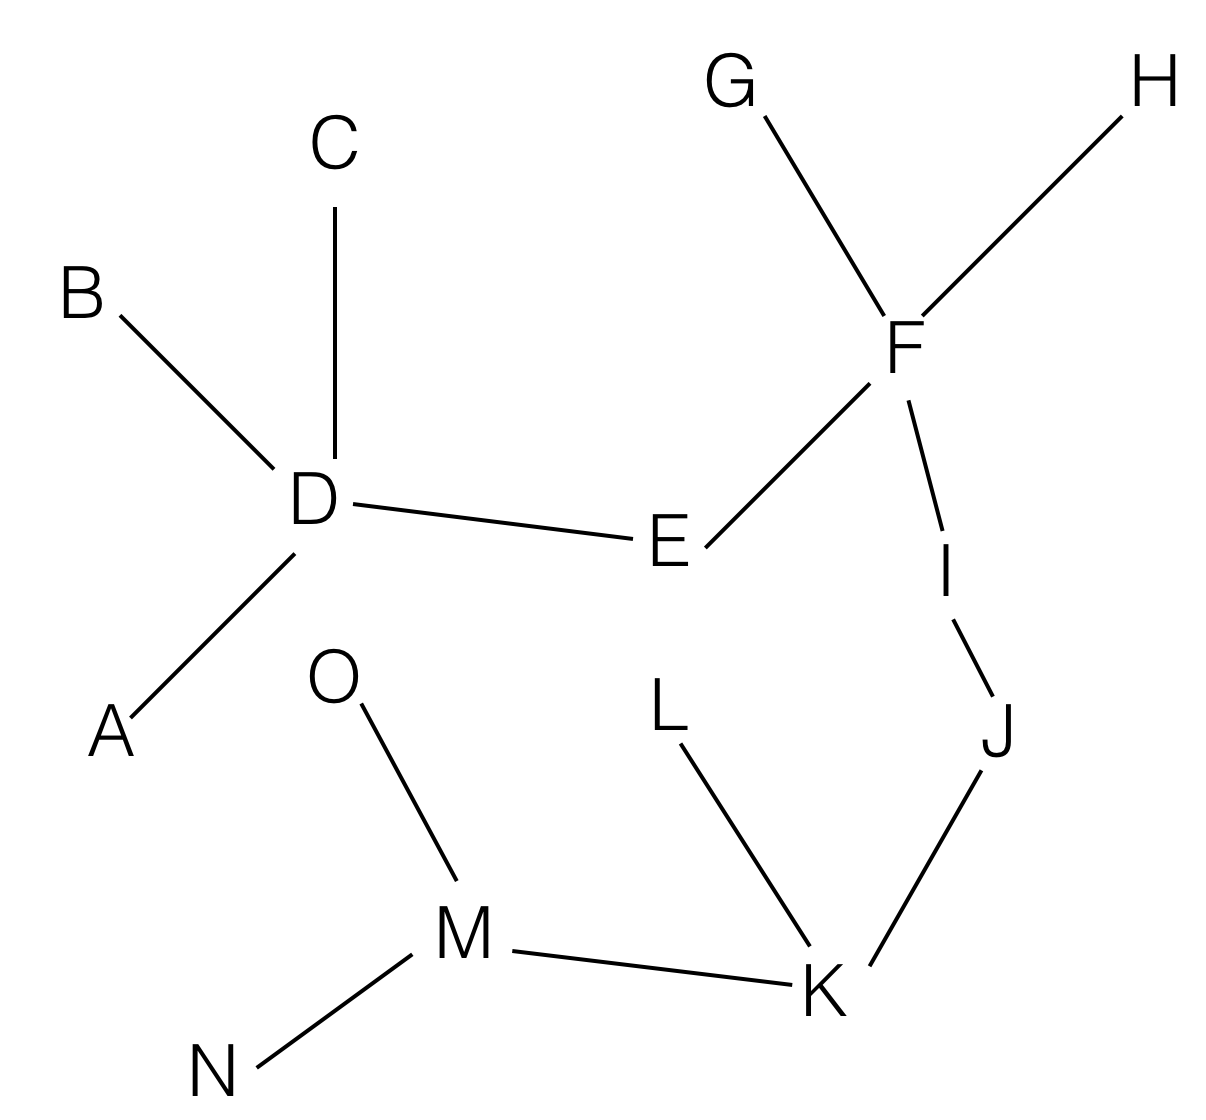
\includegraphics[width=.6\linewidth]{BC}

2. Now, input the graph into mathematica. Find which nodes have the highest betweenness centrality (if you named your graph $g$, you can input "BetweennessCentrality[g]"). Was your guess correct?
\\
\\
\\
3. Plot the degree distribution...Does it look more like a graph from the ER model or a graph from the BA model?
\\
\\
\\
\end{exercise}

\subsection{Community Detection}
The last thing we will learn about here is community detection in graphs. Often, when confronted with data, we look for some kind of underlying structure and organization to the data---what parts of the data cluster together? Are there groups of similar data points, or does everything seem random? A powerful method for deducing structure is \emph{community detection}. This can be used in many applications---for example, to find cofunctioning units of neurons within the brain, to find social cliques from Facebook data, to find voting blocs in Congress, to find organization from criminal ties (see Figure \ref{crime}), etc.
\begin{figure}[htbp]
\begin{center}
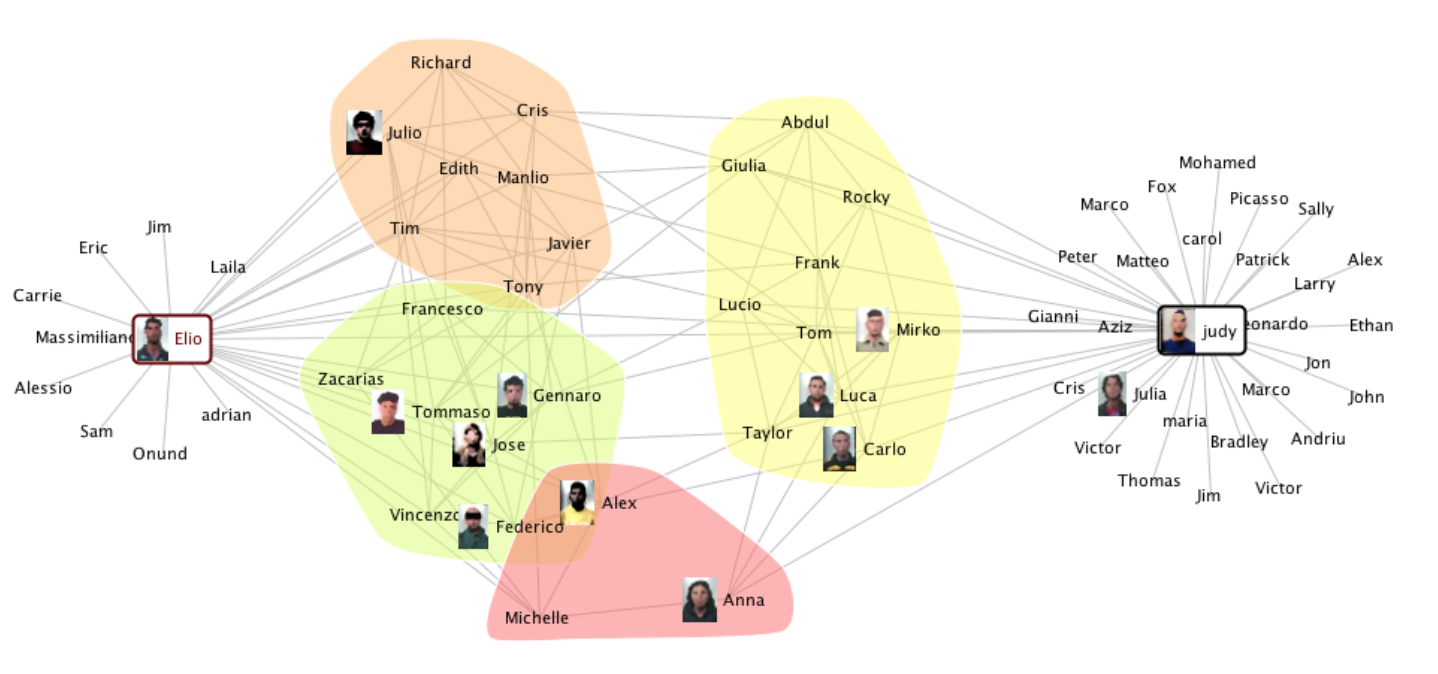
\includegraphics[width=.8\linewidth]{crime}
\caption{Network Information Reconstructed from records of cell phone calls between frequent offenders, \emph{from Prof. Emilio Ferrarra's personal webpage}}
\label{crime}
\end{center}
\end{figure}
\\Often, community organization is easy to see in data. But some networks have millions (or more) of nodes and edges---even in smaller networks, community organization may be difficult to see if the graph layout is poor. Indeed, community detection is a very active area of research, particularly here at UNC. One method is \emph{modularity}-based community detection. Like algorithms, this method relies upon optimizing (trying to increase) the output of a particular function. Intuitively, this function represents \emph{how well a certain community structure fits the given data.} 
\\In mathematica, input "g=ExampleData[\{"NetworkGraph","ZacharyKarateClub"\}]"---this data (frequently used in the community detection literature) represents a social network wherein nodes represent people and edges represent friendships within a karate club. Now input "FindGraphCommunities[g,Method$->$"Modularity"]" and then "HighlightGraph[g,Subgraph[g,\#]\&/@\%,GraphHighlightStyle$->$"DehighlightHide"]" to see the communities in this network.
\end{document}
